% !TeX root = ../BA_main_englisch.tex
% !TeX spellcheck = en_GB
We apply the methodology of Section \ref{n_5_ml} to the case of $\Delta \mathrm{T} = 1$ with 5 Drive and Transducer qubits.
Contrary to $\Delta \mathrm{T} = 5$, the optimal System states cannot be reached, leading to a lower total work output following the protocol determined by the optimiser (Figure \ref{dt_dep}).

We train the LSTM networks from Section \ref{n_5_ml} as well a network with a larger cell state dimension to match the amount of trainable parameters of the Bidirectional LSTM.
The performance of each network is listed in Table \ref{effdt1}.
We find that all networks perform better than their $\Delta \mathrm{T} = 5$ counterparts.

\begin{table}[h]
	\centering
	\begin{tabular}{ c | c | c | c }
		Network Architecture & $\eta_{test} \ [\%]$ & $\mathrm{MSE}_{test}$  & \# Parameters \\
		\hline
		Bidir. LSTM & 97.4 & 0.0238 & 7,700,222 \\
		Unidir. LSTM & 70.1 & 0.0638 & 3,206,990 \\
		Unidir. LSTM, higher cell state dimension & 69.9 & 0.0637 & 7,704,062 \\
	\end{tabular}
	\caption{Efficiencies $\eta$ and MSE loss on the test set for differing model architectures for $N=5, \Delta \mathrm{T} = 1$.}
	\label{effdt1}
\end{table}


\begin{figure}
	\centering
	\begin{subfigure}{0.85\textwidth}
		\centering
		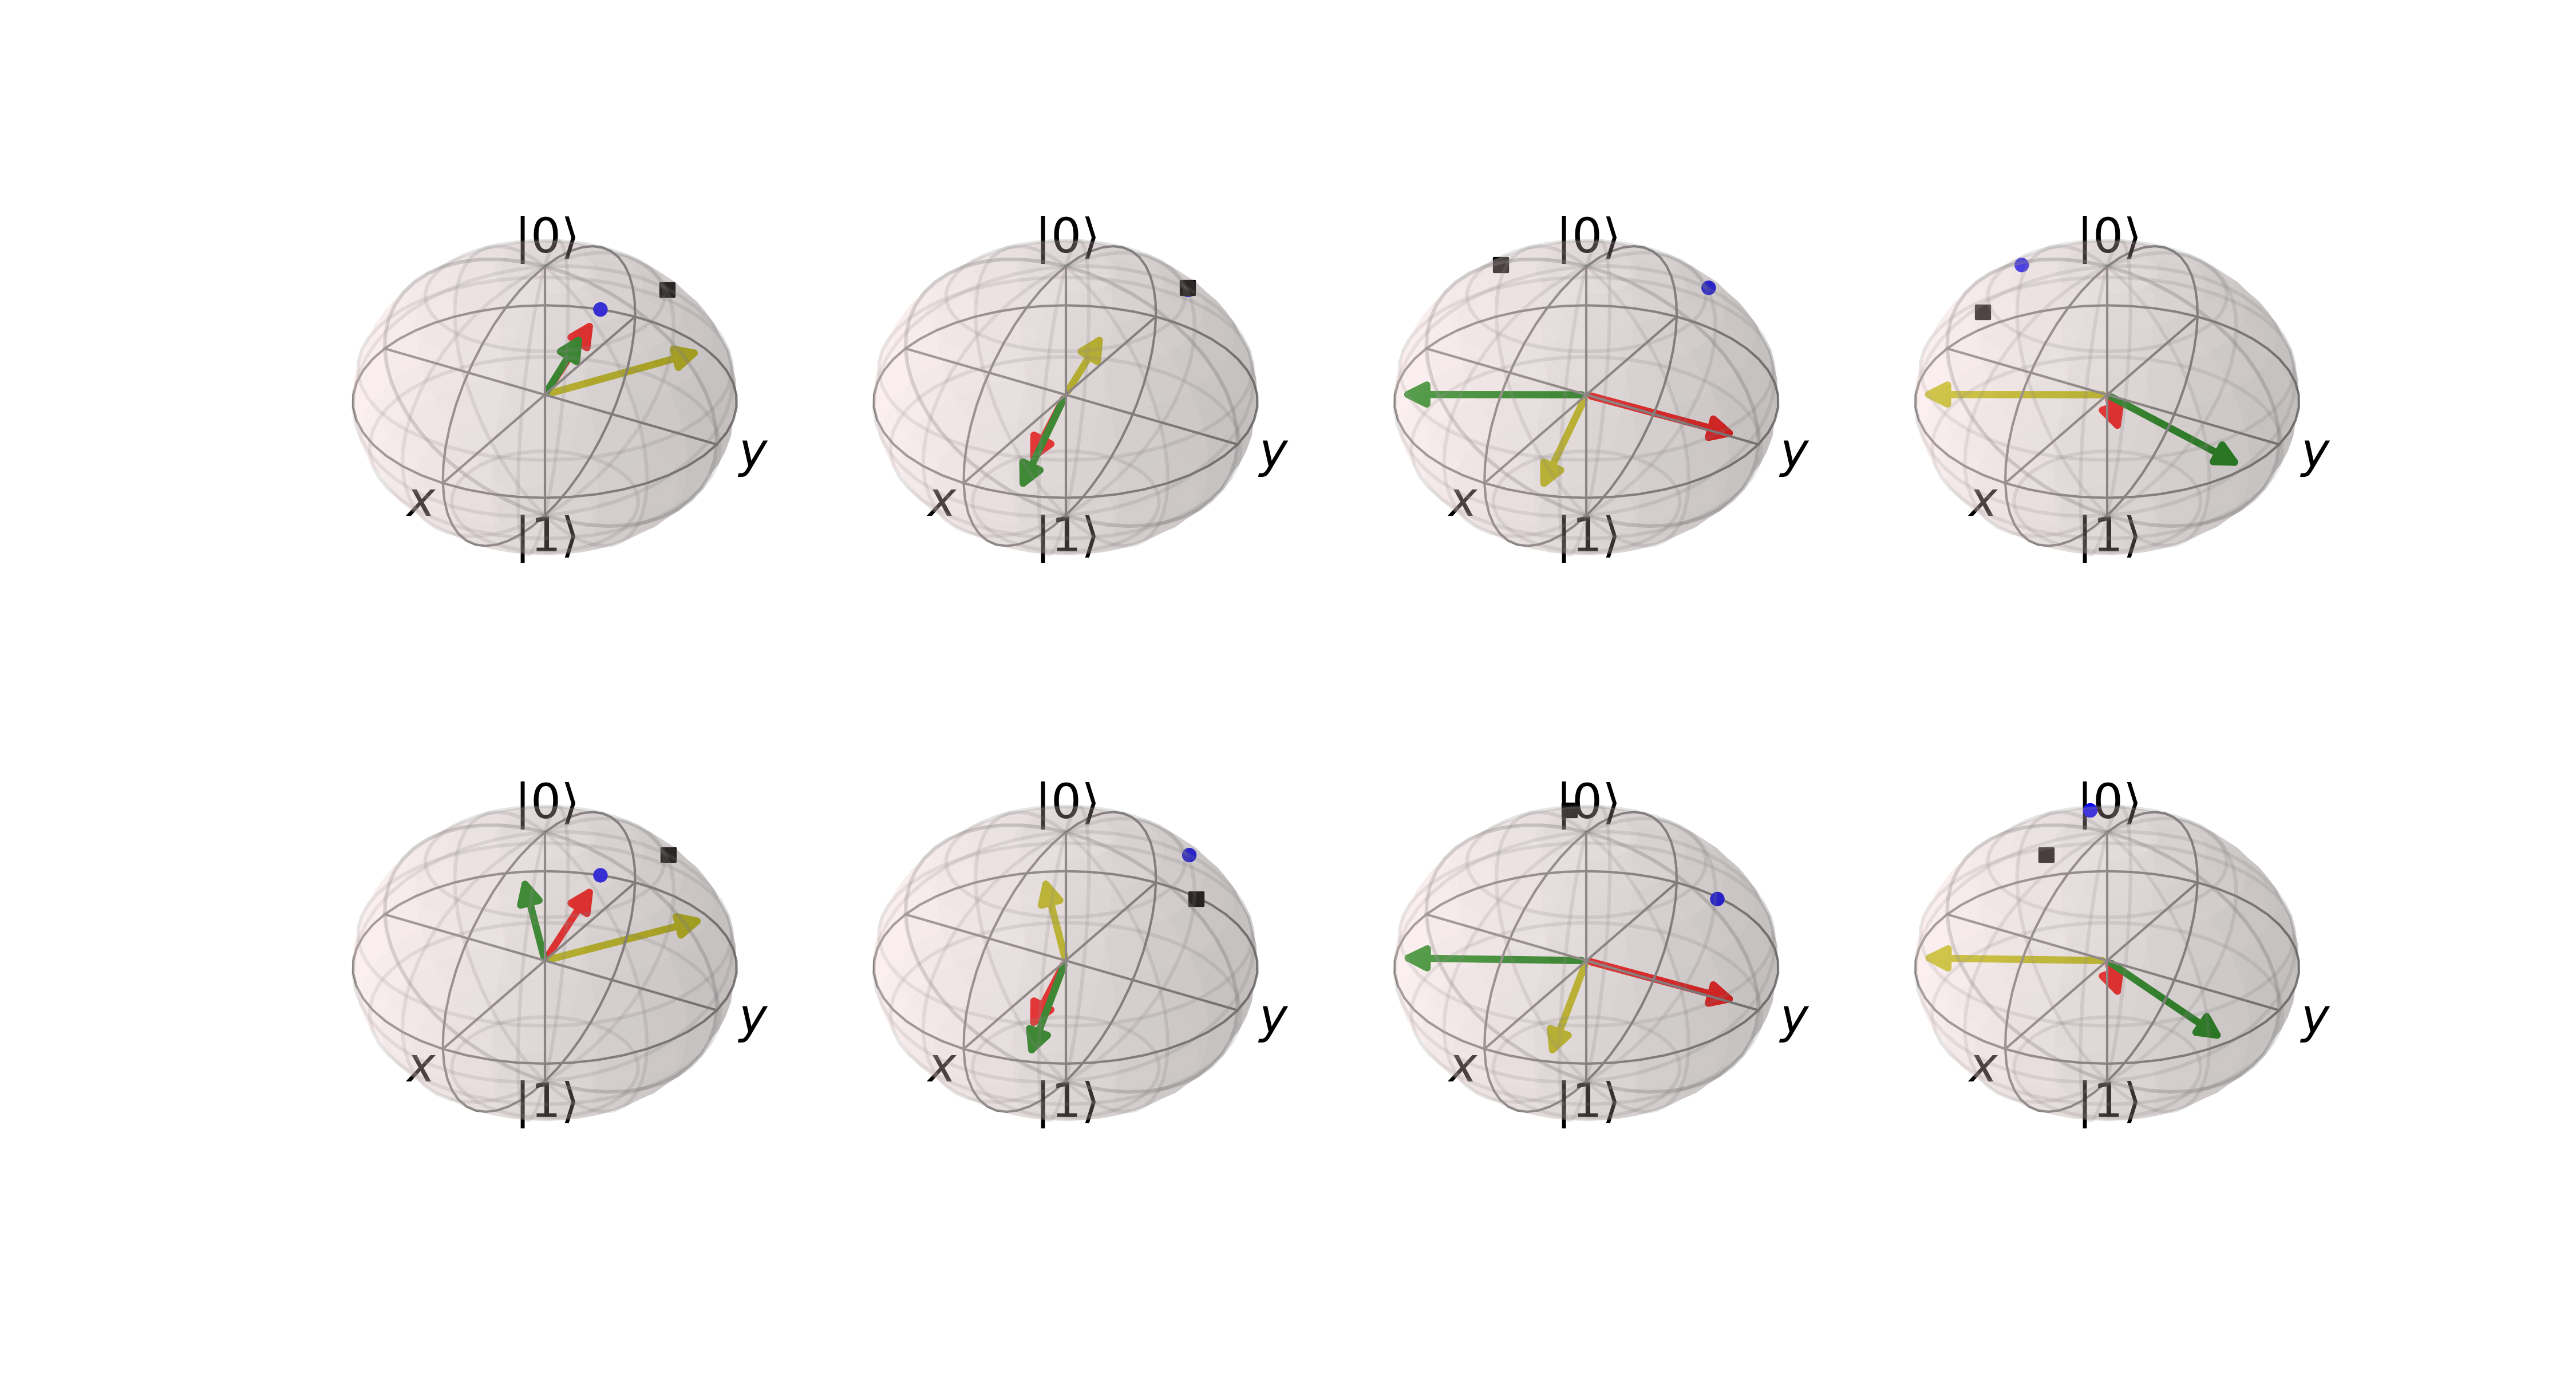
\includegraphics[width=\textwidth]{img/bloch_comp_1}
		\caption{$\Delta \mathrm{T} = 1: W_{opt} = 1.40, W_{pred} = 1.32$}
		\label{}
	\end{subfigure}
	\begin{subfigure}{0.85\textwidth}
		\centering
		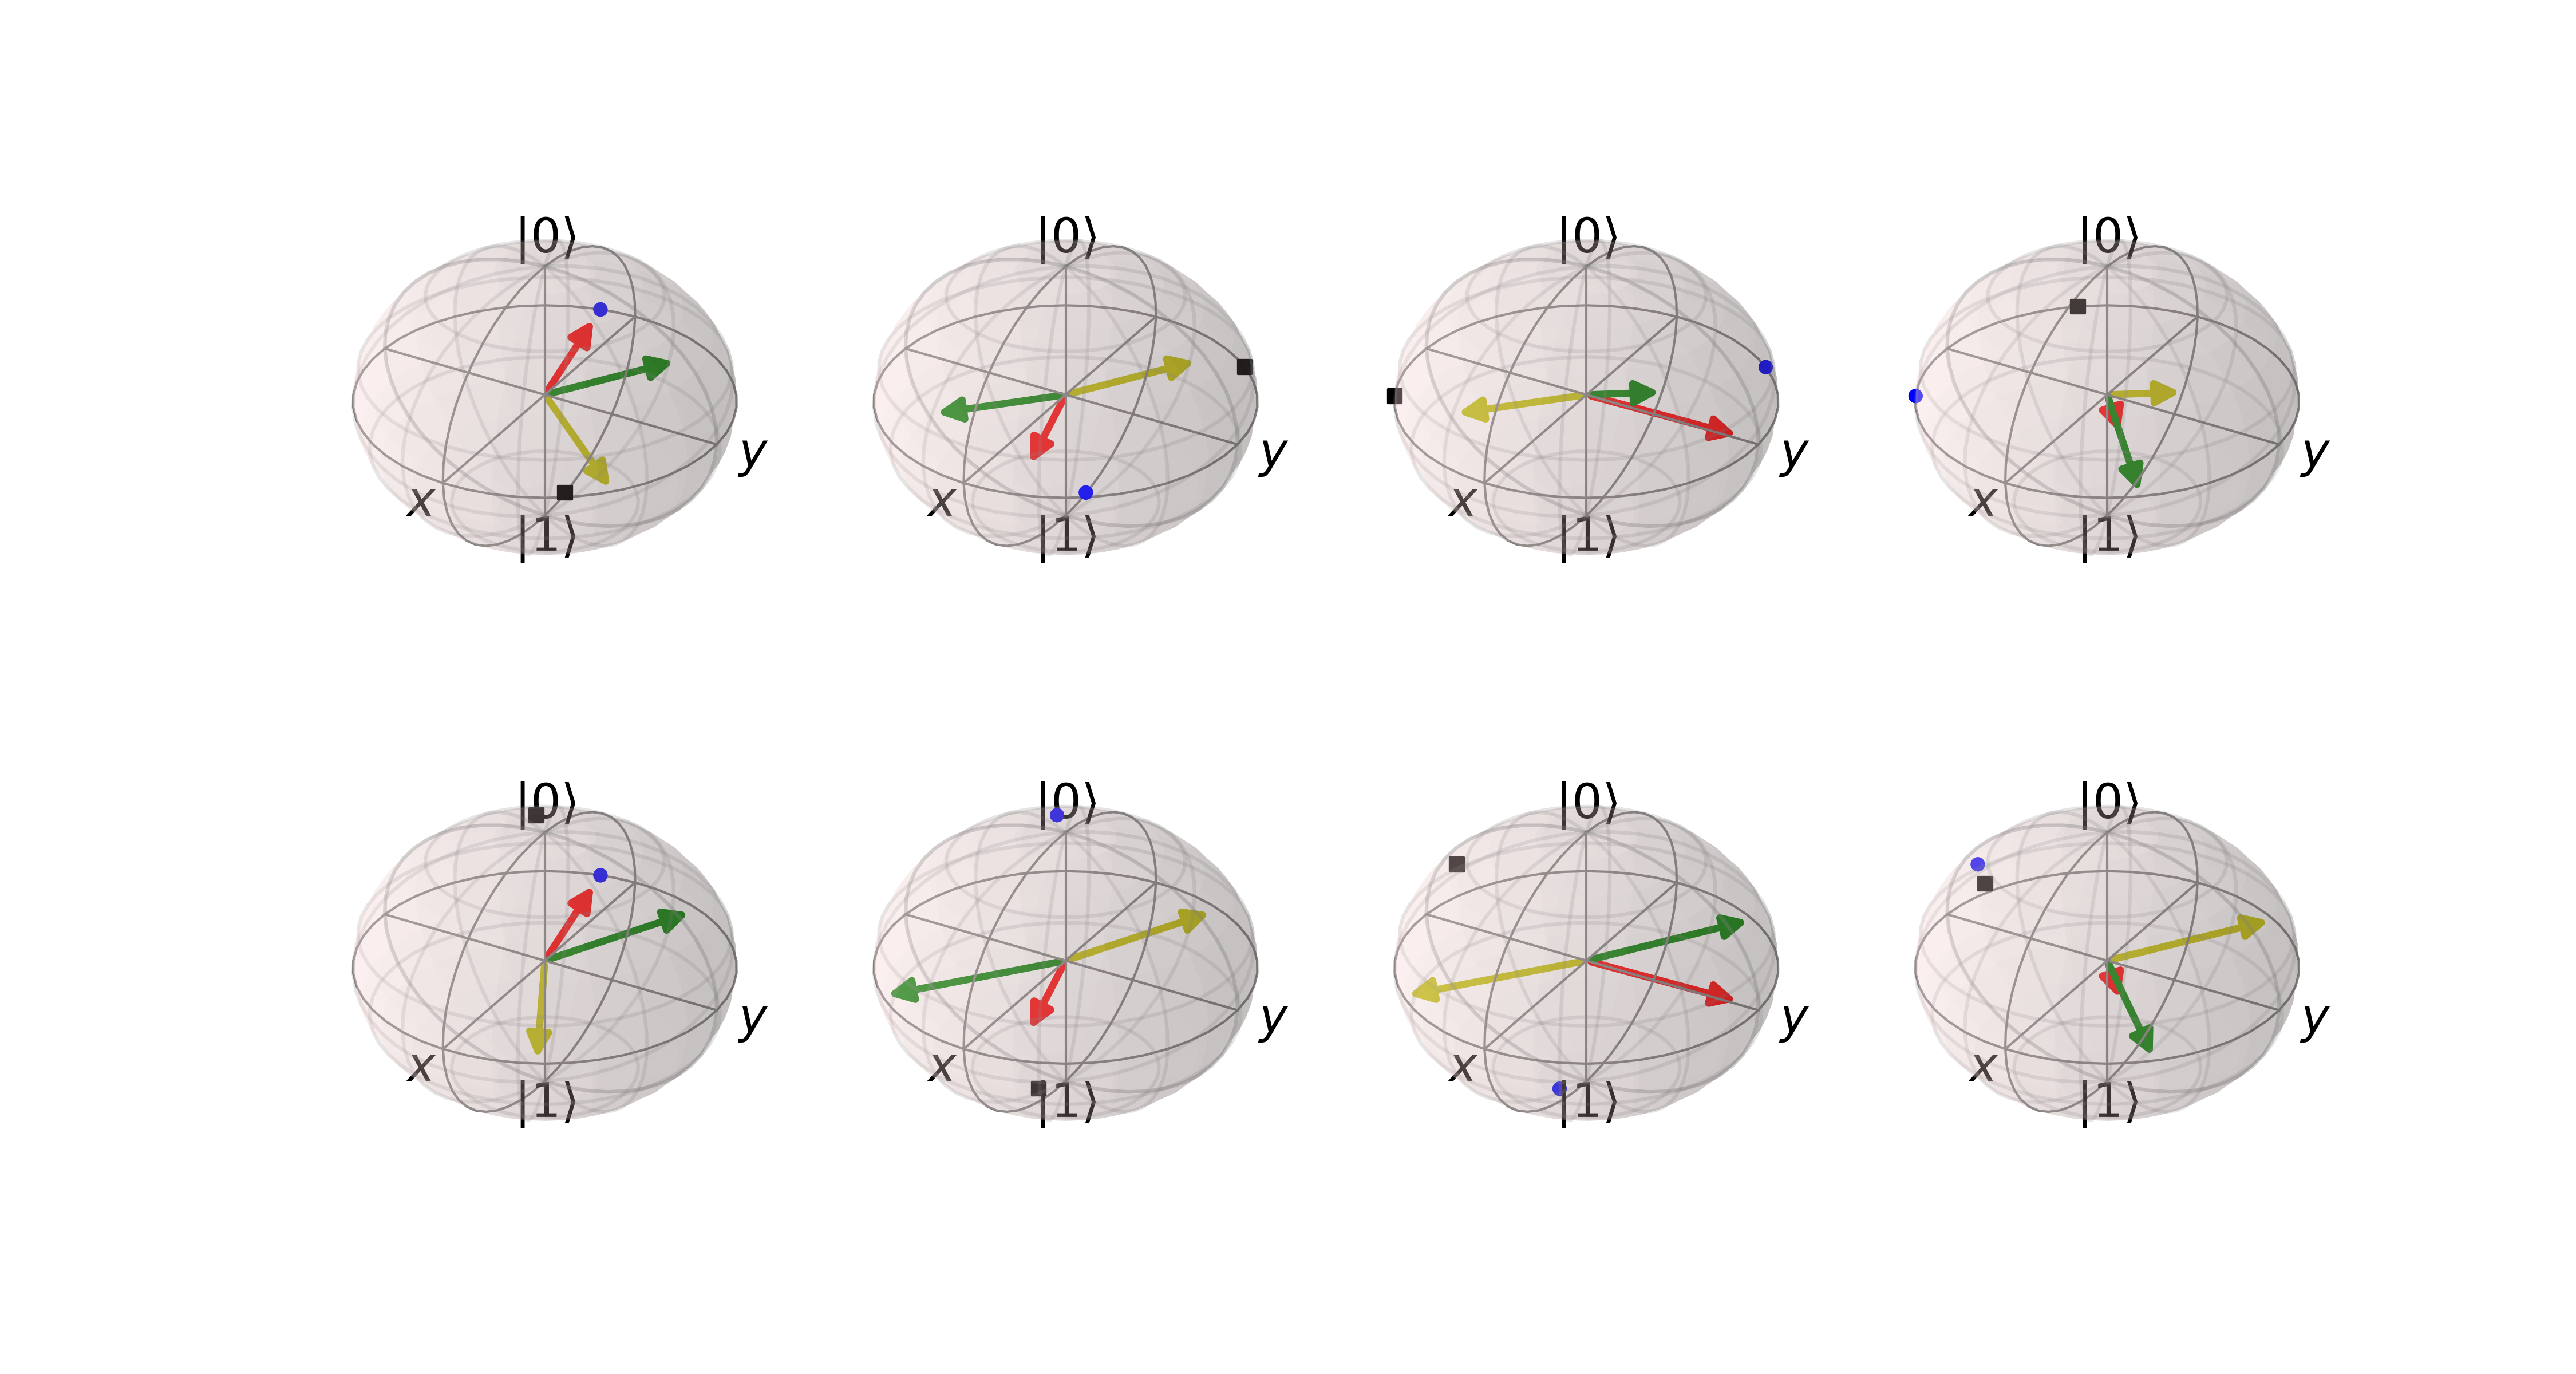
\includegraphics[width=\textwidth]{img/bloch_comp_5}
		\caption{$\Delta \mathrm{T} = 5: W_{opt} = 2.42, W_{pred} = 0.57$}
		\label{}
	\end{subfigure}
\end{figure}